\documentclass[12pt, a4paper]{article}
\usepackage{amsmath, amsfonts}
\usepackage[utf8]{inputenc}
\usepackage[russian]{babel}
\usepackage{graphicx}
\usepackage{tikz}
\usepackage{xcolor}
\usepackage{wrapfig}
\usepackage{float}
\usepackage{geometry}
\usepackage[indentfirst,compact,topmarks,calcwidth,pagestyles]{titlesec}
\usepackage{verbatim}
\usepackage{titletoc}
\usepackage{cmap}
\textheight=24cm
\textwidth=16cm
\oddsidemargin=5mm
\evensidemargin=-5mm
\marginparwidth=36pt
\topmargin=-1cm
\footnotesep=3ex
\raggedbottom
\tolerance 3000
\clubpenalty=10000
\widowpenalty=10000
\usepackage[T2A]{fontenc}
\usepackage{hyperref}
\usepackage{psfrag}

\newcommand\todo[1]{\marginpar{\textcolor{red}{#1}}}

\DeclareMathOperator*{\argmax}{argmax}
\DeclareMathOperator{\weight}{weight}
\DeclareMathOperator{\score}{score}
\DeclareMathOperator{\simu}{sim}
\DeclareMathOperator{\Dir}{Dir}
\DeclareMathOperator{\DP}{DP}
\DeclareMathOperator{\svert}{\,\vert\,}

\usepackage[ruled, linesnumbered]{algorithm2e}
\SetKwInput{KwData}{Исходные параметры}
\SetKwInput{KwResult}{Результат}
\SetKwInput{KwIn}{Входные данные}
\SetKwInput{KwOut}{Выходные данные}
\SetKwIF{If}{ElseIf}{Else}{если}{тогда}{иначе\ если}{иначе}{конец\ условия}
\SetKwFor{While}{до\ тех\ пор,\ пока}{выполнять}{конец\ цикла}
\SetKw{KwTo}{от}
\SetKw{KwRet}{возвратить}
\SetKw{Return}{возвратить}
\SetKwBlock{Begin}{начало\ блока}{конец\ блока}
\SetKwFor{For}{цикл}{выполнять}{конец\ цикла}
\SetKwFor{ForEach}{для\ каждого}{выполнять}{конец\ цикла}
\SetKwRepeat{Repeat}{повторять}{до\ тех\ пор,\ пока}
\SetAlgorithmName{Алгоритм}{алгоритм}{Список алгоритмов}

%\psfrag{all}{все}
%\psfrag{topic-specific}{тематические}

\begin{document}

Титульный лист\newpage

\tableofcontents\newpage

  \section{Введение}
  	В современном мире информация быстро устаревает, поэтому способы вовремя находить нужные данные --- постоянный объект для исследований. Одним из направлений в этой области является извлечение данных из микроблоггинговых платформ.
  	
  	Платформы микроблогов стали очень популярным способом размещения данных в Сети. В них можно найти сообщения пользователей практически на любую тему, начиная стихийными бедствиями и заканчивая рейтингами музыкальных исполнителей. Правильная обработка доступной информации --- нетривиальная задача, которая имеет множество областей применения. Последние несколько лет эта тема активно исследуется во многих университетах мира.
  	
	Отслеживание сообщений о стихийных бедствиях в реальном времени поможет вовремя организовать спасательные операции и сохранить жизни людей\cite{nuggets}. Руководствуясь сообщениями пользователей микроблогов можно судить о популярности товаров и вовремя принимать экономически целесообразные решения. Можно делать предположения о рейтингах политических деятелей и эффективности рекламы на основании информации в микроблогах. Помимо перечисленных способов применения доступной информации в микроблоггинговых платформах можно привести множество других.
	
	В данной работе в дальнейшем будет рассматриваться сервис микроблогов Твиттер\footnote{http://www.twitter.com}. В нем помимо текстовой информации можно публиковать фото, видео и геотеги, что так же может быть использовано при анализе, но в этой работе не рассматривается. В доступном наборе данных можно проводить анализ разных сущностей, эта работа посвящена выявлению событий среди потоков информации. Поскольку трактовка событий в сообщениях микроблогов может быть субъективной, выделим несколько свойств, которыми характеризуется событие.
	
	Событие в первую очередь должно быть чем-то аномальным на фоне остальных данных. Оно определяется резким изменением частотных характеристик некоторых слов в сообщениях. События в микроблогах носят взрывной характер, в течении нескольких часов частоты релевантных слов возрастают в десятки раз и так же быстро опускаются до нормального уровня. Примером события могут быть: стихийное бедствие, выход спорного законопроекта на резонансную тему, получение фильмом награды на кинофестивале.
	
	Исторически подходы к описанной задаче менялись, в следующем разделе будет рассмотрена формальная постановка задачи и эволюция способов ее решения.
	
  \section{Описание задачи}
	Цель данной работы состоит из нескольких частей:
\begin{itemize}
\item исследовать существующие подходы по извлечению событий из сети Твиттер,
\item исследовать возможность применения тематических моделей для решения описанной задачи,
\item разработать метод для извлечения событий на основе иерархического процесса Дирихле,
\item продемонстрировать работу алгоритма на реальных данных.
\end{itemize}	  
  
  Объект изучения этой работы --- алгоритм, который по входным данным строит множество событий. В качестве данных для задач подобного рода служит мультимножество документов (сообщений):
\begin{equation}
  \Omega = \left\{D_i \svert i \in \overline{1,n} \right\}.
  \end{equation}  
  Будем считать, что каждый документ имеет временную метку $t$. Документ $D_i$ определяется как упорядоченный набор слов:
\begin{equation}
  D_i = \left\{w_j \svert j \in \overline{ 1, l_i } \right\},
  \end{equation}  
   при этом слова в документах принадлежат некоторому словарю $V$. 
  
  Событие --- некоторая сущность, которая характеризуется временем возникновения и ключевыми словами. Оно вызывает резкий подъем частотных характеристик некоторых слов. Событием может быть футбольный матч и музыкальный концерт. В социальной сети Твиттер есть популярные темы, которые всегда содержат много сообщений. Например это сообщения с ключевыми словами iphone и ipad. Но такие сообщения нельзя считать событиями. Также событиями нельзя считать еженедельные пятничные сообщения о конце рабочей недели\cite{waim13}.
  
  Особенности социальной сети Твиттер состоят в следующем:
  \begin{itemize}
  \item короткие сообщения (до 140 символов),
  \item наличие шума и ошибок,
  \item большая плотность сообщений.
  \item взрывной характер событий,
  \end{itemize}
  
  \section{Анализ существующих подходов}
  Прежде чем составлять решение задачи были изучены уже существующие подходы. Все они комбинируют техники машинного обучения, обработки текстов, вероятностных графических моделей и других разделов науки. Разные методы хорошо работают для одних данных и плохо для других, на их качество также сильно влияет природа данных. Выделим несколько подходов, для того чтобы показать общую схему подобных алгоритмов и чтобы выделить идеи, повлиявшие на алгоритм, предложенный автором этой работы.
  
  \todo{сделать введение и заключение к каждому методу}
  
  \subsection{NED}
  \label{ned-subsection}
	Исторически первым подходом к извлечению событий принято считать NED (New Event Detection)\cite{ned}. NED предназначен для того, чтобы находить первый документ на тему, которая не встречалась раньше. Следующие документы на эту тему уже не будут новыми и не будут помечены алгоритмом. Для того, чтобы отвечать на вопрос, является ли документ новым, необходимо указать способ как определять степень сходства двух документов.
	
\begin{figure}[H]
  \centering
  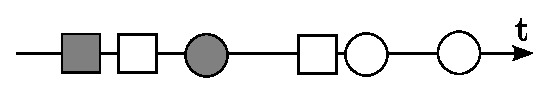
\includegraphics[width=0.58\textwidth]{ned.eps}
  \\
  \caption{Документы, соответствующие двум разным темам. Новые документы помечены серым цветом.}
  \end{figure}  

	Для этого в алгоритме NED используется техника Incremental TF--IDF (Term Frequency -- Inverse Document Frequency). TF--IDF --- базовый метод выяснять насколько отдельно взятые слова характеризуют весь документ, другими словами, насколько большой вес имеет слово $w$ в документе $d$. Пусть $f(d,w)$ --- количество слов $w$ в документе $d$. Определим значение $df_t(w)$ как количество документов, поступивших не позднее времени $t$, в которых встречается слово $w$. Используя введенные величины, можно записать значение веса определенного слова $w$ в документе $d$. В момент времени $t$ имеем:
	\begin{equation}
	\weight_t(d,w) = \frac{1}{Z_t(d)}f(d,w) \cdot \log \frac{N_t}{df_t(w)},
	\end{equation}
	где $N_t$ --- общее количество документов, поступивших не позднее времени $t$, $Z_t(d)$ --- нормализационное значение:
	\begin{equation}
	Z_t(d) = \sqrt{\sum_w \left[ f(d,w) \cdot \log \frac{N_t}{df_t(w)} \right]^2}
	\end{equation}.
	
	Теперь можно записать значение похожести двух документов, $q$ и $d$:
	\begin{equation}
	\simu_t(d,q) = \sum_w \weight(w, d) \cdot \weight(w, q).
	\end{equation}
	Указанные формулы записаны в косинусной метрике, также могут быть использованы метрики Хеллингера, Кульбака--Лейблера и другие.
	
	Для того, чтобы понять, является ли добавленный в момент времени $t$ документ $q$ новым, необходимо вычислить степень его похожести со всеми предыдущими документами. Пусть $d^*$ --- документ, максимально похожий на $q$:
	\begin{equation}
	d^* = \argmax_d \simu_t (d,q).
	\end{equation}
	Тогда значение
	\begin{equation}
	\score_t(q) = 1 - \simu_t (d^*, q)
	\end{equation}
	может быть использовано для того, чтобы определить, является ли документ $q$ новым. Новыми будем считать все документы $q$, у которых значение $\score_t(q)$ больше, чем пороговое значение $\theta_s$. В обратном случае считается что существует документ $d^*$, достаточно похожий на $q$ и поэтому $q$ не представляет собой сообщение на новую тему. Для того, чтобы определить подходящее значение $\theta_s$, можно использовать размеченный корпус и посчитать значение $\simu_t (d,q)$ среди документов, соответствующих одному и разным событиям.
	
	\subsection{Выявление событий с помощью LDA}
  На следующем примере рассмотрим как тематические модели (topic models) могут быть использованы для задачи распознавания событий. Для этого опишем схему, по которой работает алгоритм, предложенный в \cite{mediaeval}. Задача состоит в том, чтобы по данным к фотографиям Flickr\footnote{http://www.flickr.com} распознать все события на определенную тему, проходившие в конкретных городах. Фотографии содержат описания, которые можно считать документами. Основная задача может быть разбита на пять частей: 
  \begin{enumerate}
  \item предобработка данных,
  \item извлечение города,
  \item распознавание темы,
  \item распознавание события,
  \item оптимизация описания события.
  \end{enumerate}
  
  В качестве предобработки, авторы предлагают выполнить следующее: удалить стоп-слова и html теги, провести стемминг слов\footnote{стемминг (stemming) --- удаление окончаний у слов для нормализации}, перевести не английские слова на английский язык используя сервис Google Translate.
  
	Так как задача упоминает отдельные города, необходимо научиться распознавать город по документу. Географические координаты были доступны авторам в 20\% фотографий, из этих координат были выявлены города используя сервис Google Tables. Используя технику TF--IDF, в описаниях фотографий с известными городами были извлечены ключевые слова. По этим ключевым словам, появилась возможность назначить фотографиям без геотегов "ближайший" город с точки зрения похожести описаний. Для того чтобы определять похожесть документов, можно воспользоваться подходом, описанным в~(\ref{ned-subsection}). В случаях, когда "ближайший" город выявить не удалось, авторами использовались следующие предположения: считалось что один и тот же автор не мог побывать в один день более чем в двух разных городах, и что путешествие из одного города в другой занимает как минимум два часа. Эти эвристики позволили улучшить классификатор, таким образом более 97\% фотографий были привязаны к городу.
	
	Далее необходимо для каждого города кластеризовать документы по темам и рассмотреть только те из них, которые даны в описании задачи. Для распознования тем была использована тематическая модель LDA (Latent Dirichlet Allocation)\cite{lda-model}, для определения параметров которой применялось сэмплирование по Гиббсу\cite{lda-gibbs}. LDA работает из предположения, что каждый документ $d_i$ характеризуется случайным распределением над темами, в то время как каждая тема является мультиномиальным распределением над словами.
	
	Оставшаяся часть --- извлечение событий и их оптимизация. Для того чтобы алгоритм выявил событие, отвечающее теме $k$ в день $D$, необходимо чтобы количество документов $d_i$ по этой теме в день $D$ превосходило некоторое пороговое значение $\theta$. Оптимизация событий подразумевает под собой объединение событий на одну тему в последовательные дни и разделение событий в разных городах.
	
	Авторы статьи тестировали алгоритм на трех разных вариантах условия задачи, в таблице~\ref{lda-table} приведены результаты по каждому из них.
	
\begin{table}[h]
	\centering
    \begin{tabular}{ | l | l | l | l | }
    \hline
    Данные & Точность & Полнота & F-мера \\ \hline
    \#1 & 80.98 & 19.25 & 31.10 \\ \hline
    \#2 & 91.21 & 77.85 & 84.00  \\ \hline
    \#3 & 90.76 & 81.91 & 86.11 \\ \hline
    \end{tabular}
    \caption{Точность, полнота и F-мера алгоритма при разных условиях задачи}
    \label{lda-table}
\end{table}

	По результатам можно видеть что в первом случае алгоритм справляется со своей задачей существенно хуже, чем в других. Авторы объясняют это тем, что в задаче \#1 необходимо было находить научные конференции, их ключевые слова нельзя ограничить конкретным набором слов, поэтому полнота алгоритма низкая. В задаче \#2, \#3 напротив удалось обозначить необходимые ключевые слова, о чем свидетельствуют результаты.
	
	\subsection{Information nuggets}
	Рассмотрим подход к извлечению событий, описанный в~\cite{nuggets}. Авторы ставят перед собой задачу составить алгоритм описания событий в социальной сети Твиттер. Были использованы данные, полученные во время торнадо Joplin в 2011 году. Данные представляют из себя сообщения пользователей, содержащие хештег \#joplin, собранные 22 мая 2011 года на протяжении нескольких часов, пока плотность сообщений не стала относительно низкой. Авторы ставили цель извлекать из потока сообщений так называемые золотые самородки информации --- короткие и информативные сообщения, описывающие происходящие события. По этой причине подход назван information nuggets.
	
	Авторы видели основную проблему в том, что даже при наличии большого количества сообщений об одном событии, ими трудно пользоваться, потому что они имеют разную природу. Например это может быть сообщение очевидца о происходящем стихийном бедствии или сообщение о перечислении правительством средств на восстановление разрушенных построек. Статья предлагает делить сообщения на пять разных категорий по степени информативности:
	\begin{itemize}
	\item\emph{Персональное}:
	информация в сообщении может быть полезна только автору и его кругу общения. Она не является интересной для людей, которые не знают автора сообщения непосредственно.
	\item\emph{Информативное (напрямую)}:
	сообщение может быть полезно людям вне круга общения автора, и эта информация написана прямым участником или очевидцем событий.
	\item\emph{Информативное (косвенно)}:
	сообщение может быть полезно людям вне круга общения автора, при этом автор пишет о том, что он слышал по телевидению, радио или любому другому источнику информации.
	\item\emph{Информативное (напрямую или косвенно)}:
	сообщение может быть полезно людям вне круга общения автора, но невозможно ответить на вопрос как автор связан с происходящими событиями.
	\item\emph{Другое}:
	сообщение или не на английском языке, или не может быть классифицировано.
	\end{itemize}
	
	В дальнейшем рассматриваются только сообщения с информативным типом, так как они наиболее вероятно содержат полезные сведения. Затем сообщения разбиваются на подтипы по направленности информации. Всего авторами использовалось 32 разных подтипа, среди которых:
	\begin{itemize}
	\item\emph{Предостережения и советы}: документ содержит предупреждение о возможном опасном происшествии.
	\item\emph{Жертвы и разрушения}: в тексте сообщается о потерях, вызванных стихийным бедствием.
	\item\emph{Сбор средств}: сообщения описывают пожертвования денег и предметов пострадавшим от чрезвычайного происшествия.
	\end{itemize}
	
	Для того, чтобы классифицировать сообщения по типам и подтипам, в алгоритме используется наивный байесовский классификатор, который предварительно тренируется на размеченных данных. В классификаторе используется большое количество свойств, бинарных, скалярных и текстовых. В таблице~\ref{nuggets-table} приведены результаты работы алгоритма на некоторых подтипах. Для тестирования использовались размеченные вручную сообщения.
	\begin{table}[h]
	\centering
	\begin{tabular}{ | l | l | l | l | }
	\hline
	Подтип & Точность & Полнота & F-мера \\ \hline
	Предостережения и советы & 0.618 & 0.598 & 0.605 \\ \hline
	Жертвы и разрушения & 0.578 & 0.645 & 0.610 \\ \hline
	Сбор средств & 0.546 & 0.632 & 0.585 \\ \hline
	\end{tabular}
	\caption{Результаты работы алгоритма information nuggets.}
	\label{nuggets-table}
	\end{table}
  
  \section{Теоретическая часть предложенного решения}
  Эта работа ставит перед собой задачу разработать алгоритм нахождения событий в потоке сообщений пользователей сети Твиттер. В качестве данных были использованы сообщения с 4 июня 2013 года по 31 июня 2013 года, содержащие в себе хэштег \#texas. Всего корпус включает порядка 240 тысяч сообщений и 1.5 миллиона слов. Приведем псевдокод алгоритма, а затем рассмотрим каждый шаг более подробно. 
  
  \begin{algorithm}[H]
  	\SetAlgoLined
  	\KwData{множество сообщений $\Omega$, параметры алгоритма $M$, $L$, $l_D$, $J$, $R$ параметры для HDP модели}
	\KwResult{для каждого события набор ключевых слов и частота сообщений по теме события}
  	в частотной характеристике сообщений из $\Omega$ найти $K$ экстремумов, пусть они соответствуют временам $t_1,t_2,\ldots,t_K$\;
  	\ForEach{$t \in \left\{t_1,t_2,\ldots,t_K\right\}$}{
  		извлечь $M$ ключевых слов из сообщений в $\Omega$ в некотором радиусе $R$ момента времени $t$\;\label{alg:keywords-extracting-1}
  		сформировать фиктивные документы $D_0 = \left\{D_0^j\right\}_{j=1}^J$, каждый из которых имеет длину $l_D$ и состоит из полученных на шаге~\ref{alg:keywords-extracting-1} ключевых слов пропорционально их весу\;
  		добавить $D_0$ к множеству $\Omega$\;
  		каждому сообщению из $\Omega$ назначить тему, с помощью модифицированной модели HDP (Hierarchical Dirichlet Process)\;\label{alg:hdp-applying}
  		пусть документам $D_0$ была назначена тема $k$, удалить $D_0$ из $\Omega$\;
  		найти частотную характеристику сообщений в $\Omega$ с темой $k$\;
  		\eIf{событие с похожей частотной характеристикой уже было найдено}{
	  		перейти на следующую итерацию цикла\;
  		}{
  			найти $L$ ключевых слов из сообщений в $\Omega$ с темой $k$\;\label{alg:keywords-extracting-2}
  			добавить ключевые слова, частотную характеристику в результат\;
  		}
  	}
  	\caption{Извлечение событий из сообщений Твиттера}
  	\label{main-algo}
  \end{algorithm}
  
  \subsection{Нахождение экстремумов}
  Понятие экстремума в этом разделе отличается от привычного определения в математическом анализе. Назовем экстремумом те точки, в которых плотность сообщений позволяет утверждать что в этот момент произошло событие. В первую очередь, понятие экстремума для задачи выявления событий должно быть локальным. С другой стороны не все локальные максимумы можно корректно обозначить как события. Задача в общем виде получила развитие в контексте обработки сигналов~\cite{peak-detection}. Существует множество методов, каждый из которых будет больше подходить к определенному типу данных. Алгоритм нахождения экстремумов может меняться вне зависимости от других составных частей исходного алгоритма. Несколько возможных подходов нахождения экстремумов для функции $f(x)$ с сеточной областью определения $X$ перечислены ниже:
  \begin{itemize}
	\item  
	Алгоритм помечает как экстремумы все точки, в которых функция достигает максимума в некотором окне, и при этом ее значение больше некоторого заранее определенного $\theta$. Опционально $\theta$ может зависеть от среднего значения функции и других статистических характеристик.
	
	\item
  	Для любых двух значений аргумента $x$ и $y$, где $x < y$ определим функции $T(x,y)$ (travel) и $R(x,y)$ (rise):
  	\begin{equation}
  	\begin{aligned}
	  	& T(x, y) = \sum_{x \leq k < y} \left\vert f(k + 1) - f(k) \right\vert, \\
	  	& R(x, y) = f(y) - f(x) + \epsilon,
	\end{aligned}
  	\end{equation}
  	где $\epsilon$ --- некоторое небольшое значение. Тогда значения $T(x, y)/R(x, y)$ соответствуют пику функции между точками $x$ и $y$. Алгоритм может находить все экстремумы, где значение $T/R$ больше некоторого порога.
  	
  	\item
  	Подход заключается в том, чтобы выделить в функции стандартную пиковую подфункцию, например функцию Гаусса. Для этого применяются согласованные фильтры. Пусть $g(x)$ --- функция Гаусса с некоторыми $\mu$ и $\sigma$:
\begin{equation}
  	g(x) = \frac{1}{\sigma \sqrt{2\pi}} \exp\left\{ -\frac{(x-\mu)^2}{2 \sigma^2} \right\}.
  	\end{equation}  	
  	Тогда можно определить степень похожести исходной функции на функцию $g(x)$:
  	\begin{equation}
  	\simu(f,g) = \frac{\left(f,g\right)}{\Vert f \Vert \cdot \Vert g \Vert}.
  	\end{equation}
  	В косинусной метрике выражение примет следующий вид:
  	\begin{equation}
  	\simu(f,g) = \frac{\sum\limits_{x \in X} f(x) \cdot g(x)}{\sqrt{\sum\limits_{x \in X}^{\,} f^2(x)} \cdot \sqrt{\sum\limits_{x \in X}^{\,} g^2(x)}}.
  	\end{equation}
  	Аналогично предыдущим случаям, будем считать что функции "похожи" если значение $\simu(f,g)$ не меньше некоторого $\theta$.
  	
  	\item
	Один из способов найти экстремумы --- применить смешанную модель (mixture model) к входной функции. Компонентами модели могут быть нормальные распределения. Затем нужно найти параметры модели используя EM алгоритм или сэмплирование по Гиббсу. Этот метод будет корректно обрабатывать случай, когда экстремумы накладываются друг на друга или расположены очень близко.
  \end{itemize}
  
  Каждый из перечисленных методов можно комбинировать со сглаживающими фильтрами если шум мешает выделить события.
  Для исходной задачи был выбран первый метод из списка. Данные показали что экстремумы сильно выделяются на фоне средней плотности сообщений и расположены на значительном расстоянии. Таким образом выбранный метод выдает приемлемые результаты.
  
  \subsection{Извлечение ключевых слов}
  Для того, чтобы использовать на шаге \ref{alg:hdp-applying} модель HDP с частичным обучением, необходимо знать ключевые слова события, которое мы хотим проследить с помощью тематической модели. Их извлечение происходит на шаге \ref{alg:keywords-extracting-1} и \ref{alg:keywords-extracting-2}. В реализации алгоритма учитывая особенности сети Твиттер был реализован наиболее простой способ извлечь $M$ ключевых слов из набора сообщений, а именно отсортировать слова по невозрастанию частоты и взять первых $M$ слов.
  
  Этот способ показал хорошие результаты потому что события в сети Твиттер носят "взрывной" характер и частота релевантных слов во время события в десятки и сотни раз превосходит нормальную частоту этих слов. В случае когда "взрывного" характера событий не наблюдается, при извлечении ключевых слов можно использовать технику TF--IDF. Также в этом случае можно рассматривать биграммы и применять различные методы NLP\footnote{Natural Language Processing --- обработка текстов на естественном языке} к анализируемому тексту.
  
  \subsection{Модифицированная модель HDP}
  Для извлечения всех сообщений, принадлежащих событию, в алгоритме используется модифицированная модель HDP , в которую добавлена возможность частичного обучения.
  
  \subsubsection{Иерархоческий процесс Дирихле}
  Пусть $(\Theta, \mathcal{B})$ --- измеримое пространство, с вероятностной мерой $G_0$. Пусть $\alpha_0$ --- положительное действительное число. Определим процесс Дирихле $\DP(\alpha_0, G_0)$ как случайное распределение вероятностной меры $G$ над $(\Theta, \mathcal{B})$, такое, что для любого конечного измеримого разбиения $\Theta$ $(A_1, A_2, \ldots, A_r)$, случайный вектор $(G(A_1), G(A_2), \ldots, G(A_r))$ будет распределен согласно конечномерному распределению Дирихле с параметрами $(\alpha_0 G_0(A_1), \alpha_0, G_0(A_2), \ldots, \alpha_0 G_0 (A_r))$:
  \begin{equation}
  (G(A_1), G(A_2), \ldots, G(A_r)) \sim \Dir(\alpha_0 G_0(A_1), \alpha_0, G_0(A_2), \ldots, \alpha_0 G_0 (A_r)).
  \end{equation}
  
  Иерархический процесс Дирихле это распределение над множеством вероятностных мер над $(\Theta, \mathcal{B})$. Процесс определяет множество вероятностных мер $G_j$, по одному на каждую группу, и глобальную меру $G_0$. Глобальная мера $G_0$ распределена согласно процессу Дирихле с параметрами $\gamma$ и базовым распределением $H$:
  \begin{equation}
  G_0 \svert \gamma, H \sim \DP(\gamma, H).
  \end{equation}
  Групповые меры $G_j$ условно независимы при заданном $G_0$ и имеют следующее распредедление:
  \begin{equation}
  G_j \svert \alpha_0, G_0 \sim \DP(\alpha_0, G_0).
  \end{equation}
  
  Гиперпараметрами HDP являются базовое распределение $H$ и концентрационные параметры $\gamma$ и $\alpha_0$.
  Иерархический процесс Дирихле может быть использован как априорное распределение над параметрами групповых данных. Для каждого $j$ пусть $\theta_{j1}, \theta_{j2}, \ldots$ --- независимые распределенные по закону $G_j$ случайные величины. Каждая величина $\theta_{ji}$ будет соответствовать наблюдаемому значению $x_{ji}$. Правдоподобие может быть записано в следующем виде:
  \begin{equation}
  \begin{aligned}
  & \theta_{ji} \svert G_j \sim G_j, \\
  & x_{ji} \svert \theta_{ji} \sim F(\theta{ji}).
  \end{aligned}
  \end{equation}
  
  Процесс, описанные выше носит название смешанная модель для иерархического процесса Дирихле (hierarchical Dirichlet process mixture model)\cite{hdp-1}.
  
  \subsubsection{Chinese Restaurant Franchise}
  HDP --- непараметрическая тематическая модель, процесс генерации данных по модели может быть описан в терминах процесса "chinese restaurant franchise" (CRF). В этом процессе существует сеть ресторана, в каждом из которых одинаковое меню. В ресторане находится неограниченное число столов, за каждым столом неограниченное число мест; каждый посетитель, заходя в ресторан, садится либо за уже занятый стол, либо за новый стол. На каждом непустом столе в ресторане заказано одно блюдо из меню, которое едят все посетители, сидящие за этим столом. Блюдо на стол заказывает первый человек, севший за этот стол.
  
  В CRF группам соответствуют рестораны, а параметры $\theta_{ji}$ считаются посетителями. Переменные $\phi_1, \ldots, \phi_K$ составляют единое меню для сети ресторанов, эти переменные распределены согласно базовому распределению $H$. Пусть $\psi_{jt}$ --- переменная, связанная со столом $t$ в ресторане $i$ и обозначающее блюдо, которое заказано за этим столом.
  
  Каждый посетителю $\theta_{ji}$ соответствует стол $\psi_{jt}$, в то время как каждому столу $\psi_{jt}$ соответствует одно блюдо $\phi_k$. Для того, чтобы указать это соответствие, используются индексы:
  \begin{itemize}
  	\item $t_{ji}$ --- индекс, связывающий посетителя $\theta_{ji}$ со столом $\psi_{jt}$, за которым сидит этот посетитель.
  	\item $k_{jt}$ --- индекс, связывающий стол $\psi_{jt}$ с блюдом $\phi_k$, которое заказано для этого стола.
  \end{itemize}
  Для описания процесса, необходимо ввести следующие обозначения:
  \begin{itemize}
  \item $n_{jtk}$ --- количество посетителей в ресторане $j$ за столом $t$, едящих блюдо $k$;
  \item $n_{jt\cdot}$ --- количество посетителей в ресторане $j$ за столом $t$;
  \item $n_{j\cdot k}$ --- количество посетителей в ресторане $j$, едящих блюдо $k$;
  \item $m_{jk}$ --- количество столов в ресторане $j$, на которых заказано блюдо $k$;
  \item $m_{j\cdot}$ --- количество столов в ресторане $j$;
  \item $m_{\cdot k}$ --- количество столов, на которых заказано блюдо $k$;
  \item $m_{\cdot \cdot}$ --- общее количество столов.
  \end{itemize}
  
  Запишем условное распределение $\theta_{ji}$, где $G_j$ исключены интегрированием:
  \begin{equation}
  \label{eq:1}
  \theta_{ji} \svert \theta_{j1}, \theta_{j2}, \ldots, \theta_{j,i-1}, \alpha_0, G_0 \sim
  \sum \limits_{i=1}^{m_j} \frac{n_{j t \cdot}}{i - 1 + \alpha_0} \delta_{\psi_{jt}} + \frac{\alpha_0}{i - 1 + \alpha_0} G_0.
  \end{equation}
  Интегрируя по $G_0$, получим:
  \begin{equation}
  \label{eq:2}
  \psi_{jt} \svert \psi_{11}, \psi_{12}, \ldots, \psi_{21}, \ldots, \psi_{j, t-1}, \gamma, H \sim
  \sum \limits_{k=1}^{K} \frac{m_{\cdot k}}{m_{\cdot \cdot} + \gamma} \delta_{\phi_k} + \frac{\gamma}{m_{\cdot \cdot} + \gamma} H.
  \end{equation}
  
  Уравнение (\ref{eq:1}) описывает выбор стола посетителем, в то время как уравнение (\ref{eq:2}) определяет выбор блюда.
  
  Если перевести используемые термины в область тематических моделей, посетители будут соответствовать словам, рестораны документам, столы внутренним темам документов, блюда внешними темами всего корпуса\cite{hdp-1}.
  
  \subsubsection{Модификация частичной обучаемости}
  HDP является моделью без учителя, она не требует размеченных данных для того чтобы назначить документам соответствующие темы. Для того, чтобы контролировать процесс определения тем, необходимо соответствующе изменить модель. В алгоритме \ref{main-algo} необходимо добиться от HDP того, чтобы она выделила ключевые слова из некоторого множества $\mathcal{K}$ в отдельную тему $k_0$. Есть несколько способов добиться требуемого результата, один из них описан ниже \cite{ss-learning}.
  
	Составим из ключевых слов в $\mathcal{K}$ документ длины $M$, в котором количество каждого ключевого слова пропорционально его весу. Перед тем как находить параметры HDP для корпуса документов, добавим $J$ сгенерированных документов в корпус. 
	
  Для того, чтобы извлечь параметры из модели HDP в алгоритме применяется сэмплирование по Гиббсу. В этом методе изначальные документы каким-то образом распределяются по темам, а затем итеративно каждое слово удаляется из состояния и назначается на новое место, согласно уравнениям (\ref{eq:1}) и (\ref{eq:2}). Упрощенный псевдокод сэмплирования по Гиббсу для модели HDP приведен ниже:
  
  \begin{algorithm}[H]
  	\caption{Сэмплирование по Гиббсу}
  	распределелить все слова на тему 0\;
  	\Repeat{не прошло $L$ итераций}{
	  	Бубубу\;
  	}
  \end{algorithm}
  
\begin{thebibliography}{9}
	\bibitem{nuggets}
	Imran, Elbassuoni, Castillo, Diaz and Meier.
	Extracting Information Nuggets from Disaster-Related Messages in Social Media.
	2013.
	\bibitem{waim13}
	Xun Wang, Feida Zhu, Jing Jiang, Sujian Li.
	Real Time Event Detection in Twitter.
	2011.
	\bibitem{ned}
	Thorsten Brants, Francine Chen, Ayman Farahat.
	A System for New Event Detection.
	2003.
	\bibitem{mediaeval}
	Konstantinos N. Vavliakis, Fani A. Tzima, and Pericles A. Mitkas.	
	Event Detection via LDA for the MediaEval2012 SED Task.
	2012.
	\bibitem{lda-model}
	David M. Blei, Andrew Y. Ng, Michael I. Jordan.
	Latent Dirichlet Allocation.
	2003.
	\bibitem{lda-gibbs}
	Tom Griffiths.
	Gibbs sampling in the generative model of Latent Dirichlet Allocation.
	\bibitem{peak-detection}
	Girish Keshav Palshikar.
	Simple Algorithms for Peak Detection in Time-Series.
	\bibitem{hdp-1}
	Yee Whye Teh, Michael I. Jordan, Matthew J. Beal, David M. Blei.
	Hierarchical Dirichlet Processes.
	2005.
%	\bibitem{hdp-2}
%	Yee Whye Teh.
%	Hierarchical Bayesian Nonparametric Models with Applications.
%	2009.
	\bibitem{ss-learning}
	Ramnath Balasubramanyan, William W. Cohen, Matthew Hurst.
	Modeling corpora of timestamped documents using semisupervised nonparametric topic models.
		
\end{thebibliography}
  
\end{document}
